\documentclass[runningheads,a4paper]{llncs}

\usepackage{amssymb}
\usepackage{amsmath}
\setcounter{tocdepth}{3}
\usepackage{graphicx}
\usepackage{subfigure}
\usepackage{url}
\usepackage{bm}
\urldef{\mailsa}\path|{qian_chen}@sjtu.edu.cn|
\newcommand{\keywords}[1]{\par\addvspace\baselineskip
\noindent\keywordname\enspace\ignorespaces#1}

\begin{document}

\mainmatter

\title{ Affective Recognition Using EEG Signal in Human-robot Interaction }
\titlerunning{ Affective Recognition Using EEG Signal in Human-robot Interaction}

\author{Chen Qian\and Tingting Hou\and Shan Fu }

\authorrunning{ Affective Recognition Using EEG Signal in Human-robot Interaction}
\institute{School of Electronic Information and Electrical Engineering, Shanghai Jiao Tong University,
Shanghai, 200240, P.R. China\\
\mailsa }

\maketitle
%Abstract
\begin{abstract}
TODO : this part is waiting to be rewritten.
\keywords{Affective Computing; Arm-Robot Operation; Time Domain Features;
Domain Feat}
\end{abstract}

\section{Introduction}
Hitherto, mechanical arm, as a vital product in industry field, has been broadly
used in medical, exploration, rescue field etc. However, the mistaken operation
caused by human error, which should have been avoided, is still one of the
dominant reasons causing accidents. As we all know, the performance of human has a
close link to the cognitive state of human and to some degree emotion is the
main reason causing the change of the cognitive state. Therefore, one of the
critical ways to avoid huamn error in mechanical arm operation is recognizing
the emotion during the opreration process through detecting the physiological
signal. Since R. W. Picard has defined $Affective\ Computing\ (AC)^{\cite{AC}}$
in 1995, affective computing has been a critical field in human-computer
interaction area. There are numerous physiological signals which could reflect
the cognitive state of human, such as Blood Volume Pressure (BVP), Skin Conductance
Response (SCR), Respiration (RESP), Electrocardiogram (ECG), Electromyogram (EMG),
Electrocorticogram (ECoG), Electroencephalogram (EEG), Heart Rate (HR), Oxygen
Saturation (SaO2) and Surface Temperature (ST)\cite{KR}. In all physiological
signals, EEG is no doubt the most capable signal directly reflecting the brain
activity. Therefore this paper chooses to use 32 dry electrodes EEG signal acquisition
equipment to obtain EEG signal data during mechanical arm operation.


There are lots of models which have been proposed to describe the emotion, such as
six basic emotions model proposed by Ekman et al.\cite{Ekman}, eight basic emotions
model proposed by Plutchik\cite{Plutchik} and the valence-arousal scale proposed
by Russell\cite{Russell}. For simplifing this problem, this paper chooses to use the
valence in the valence-arousal model of Russell to evaluate the emotion of the subjects.
And the valence reflecting the positive or negative aspect of the subjects is enough
to describe the cognitive state of the subjects.


Besides the model of emotion, the way to obatain the ground truth of the subjects cognitive state
is also crucial. Almost all research in Affective Computing field use the self-assessment
scores to estimate the true cognitive state of the subjects. However, even the subjects
themselves could hardly to retell the exact emotion state in the mechanical arm operation
and using one single scores to estimate the cognitive state during the entire operation process
 is obiviously not reasonable in detail. So this paper proposes to use objective and real time
 indexes to represent the cognitive state of the subjects. In this paper, we record the track
 of the end point of the mechanical arm and extract the features of the track to represent
 the fluctuation of the cognitive state of the subjects. Meanwhile, we assume that the workload
  and the time pressure could stimulate the emotion change of the subjects, so we give a
  basic score, which reflects the emotion state the subjects should be, and add the weighted
  features scores to the basic score to reflect the fluctuation of the emotion state.


In our experiment, we designed three levels of operating tasks in different difficulty to
  stimulate the emotion state change. And the level of difficulty is determined by the
  workload and the time pressure. To eliminate the influence of unfamilarity, one minute
  of free exploration is added before these three tasks and to eliminate the interaction
  of different tasks, a 30 seconds reset time interval is added between the different
  tasks.


During the data process part, because of the low signal-to-noise ratio (SNR),
the disturbance of EMG signal and the electromagnetic interference, the raw data
have firstly been filter to the 1-64Hz frequecy band\cite{Feature}. After normalization
process, different scales sliding window are induced in extracting features. Because of
the real-time label we obtain from the track mentioned above, it allows us to consider the
data in single sliding window as one sample.

The feature extraction methods are detailed summarized in papaer\cite{Feature}, we choose
three time domain features and one frequency feature to represent the raw data according
to the value of the weighted relative occurrence. And at the feature selection process,
we apply Principal Component Analysis (PCA) and Linear Discriminant Analysis (LDA) to
select the extracted features above. And at the classification design process, we apply
Support Vector Machine (SVM), which is a effective classification discriminator,
to predict the emotion state.

Here is the remainder organization of this paper: Section 2 introduce the
apparatus used in the experiment and the detail experiment protocol. Section 3
describes the data preprocess procedure, feature extraction, feature selection
classification design methods. Section 4 focus on showing the data process
results. Section 5 discusses the results. Section 6 gives the conclusion of
our experiment.
%mistake, Emotion is an important psychological process which could be induced by
%conscious and unconscious brain activities. This psychological process could
%reflect the cognitive state of , such as emotional images, musics, and video clips.
%Actually, many researching works have been done

\section{Experiment Setup}
\subsection{Apparatus}
There are 3 key equipments we use in our experiment: EEG Signal Acquisition Equipment,
Mechanical Arm and Joystick. And there are 3 personal computers for communicating
with EEG equipment, controling movement of mechanical arm through joystick and
showing the end point of the mechanical arm.
\paragraph{EEG Signal Acquisition Equipment:}
The EEG Signal Acquisition Equipment we apply is the $Cognionics\ HD-72\ Dry\ EEG
\ Headset^{\cite{cognionics}}$ (see in Fig.~\ref{fig:EEGequipment}).
Considering the difficulty of wearing EEG equipment and the comfort of the subjects,
we choose 32 dry electrodes, according to the international 10-20 system,
to obtain the EEG signal, which are showed in Fig.~\ref{fig:sensorloc}.
The sampling rate is 500Hz which is sufficient for obtaining EEG signal.
\begin{figure}
    \centering
    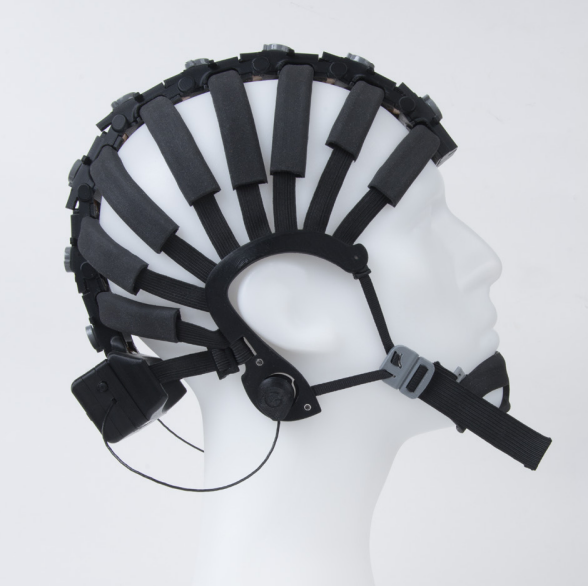
\includegraphics[height=4cm]{images/1}
    \caption{Cognionics HD-72 Dry EEG Headset}
    \label{fig:EEGequipment}
% \end{figure}
% \begin{figure}
    \centering
    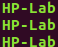
\includegraphics[height=8cm]{images/2}
    \caption{32 dry electrodes sensor location}
    \label{fig:sensorloc}
\end{figure}

\paragraph{Mechanical Arm:}
The mechanical arm we apply is the $Dobot\ Magician\ mechnical\ arm^{\cite{dobot}}$
(see in Fig.~\ref{fig:dobot}), because it supports reprogramming according to
the need of users and the control precision (0.2mm) is adequate for our experiment.

\begin{figure}
    \centering
    \includegraphics[height=4cm]{images/3}
    \caption{Dobot Magician mechanical arm}
    \label{fig:dobot}
\end{figure}

\paragraph{Joystick:}
The joystick we use is the flying joystick named $Extreme\ 3D\ Pro^{\cite{joystick}}$
produced by Logitech (see in Fig.~\ref{fig:joystick}).
The perfect ergonomic design with a custom twist-handle rudder relies
its one-handed control resulting in a smaller device footprint.
There are six programmable buttons on the base.
Each programmable button can be configured to execute simple single commands or
intricate macros involving multiple keystrokes, mouse events, and more.
In our experiment, we only operate the rocker in six basic direction movement,
which are left-right direction, front-behind direction and left-right rotation.

\begin{figure}
    \centering
    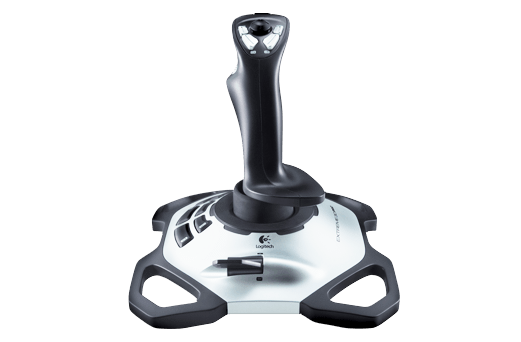
\includegraphics[height=4cm]{images/4}
    \caption{Logitech Extreme 3D Pro joystick}
    \label{fig:joystick}
\end{figure}

In our experiment, we use Robot Operating System (ROS) to receive the control
signal from joystick, release the control signal to mechnical arm, recieve the
position information of the end point of the mechnical arm and record the track
information with real time mark point in a sampling rate of 10Hz
(code url: \url{https://github.com/QCH1993/DobotMagician}). Meanwhile,
real time EEG signal are recorded with mark information which could be used in
subsequent time correcting process.

\subsection{Experiment Protocol}
Five healthy participants (two females, three males), aged between 23 and 25,
participated in the experiment. Before all experiments, all participants were
asked to have adequate sleepness.

In our experiment, firstly, participants were asked to read the experiment
procedures and notes and the experimenter would read out the procedures and notes
for a second reminder. And the experimenter was also present there to answer any questions.
At the beginning of each experiment,
one minute of free exploration were given to remove the interference caused by unfamiliarity.
And then the subjects were asked to operate the mechnical arm to touch
the different color point on the desktop according to a certain order.
We designed three levels of operating tasks in different difficulty (easy, medium and hard mode)
according to the number and position of points and the time constraint. In easy
mode, the subjects were asked to touch three colored points without time pressure.
In medium mode, the subjects were asked to touch five colored points without
time pressure. In hard mode, the subjects were asked to touch five colored points
in 90 seconds. To eliminate the interplay between the three tasks,
a 30 seconds break time for resetting was added after each task.

The experiment enviroment is showed in Fig.~\ref{fig:experiment}.
The Fig.~\ref{fig:experiment:a} is the overview of the entire experiment environment.
The subject operation platform (see in Fig.~\ref{fig:experiment:b}) is insulated
from the mechnical arm platform and
all the information helping the subjects to move the mechnical arm was from three
camera set around the mechnical arm and on the end point of the mechnical arm
(see in Fig.~\ref{fig:experiment:c}). The screen interface presenting the information from
cameras are showed in Fig.~\ref{fig:experiment:d}.

\begin{figure}
  \centering
  \subfigure[overview]{
    \label{fig:experiment:a} %% label for first subfigure
    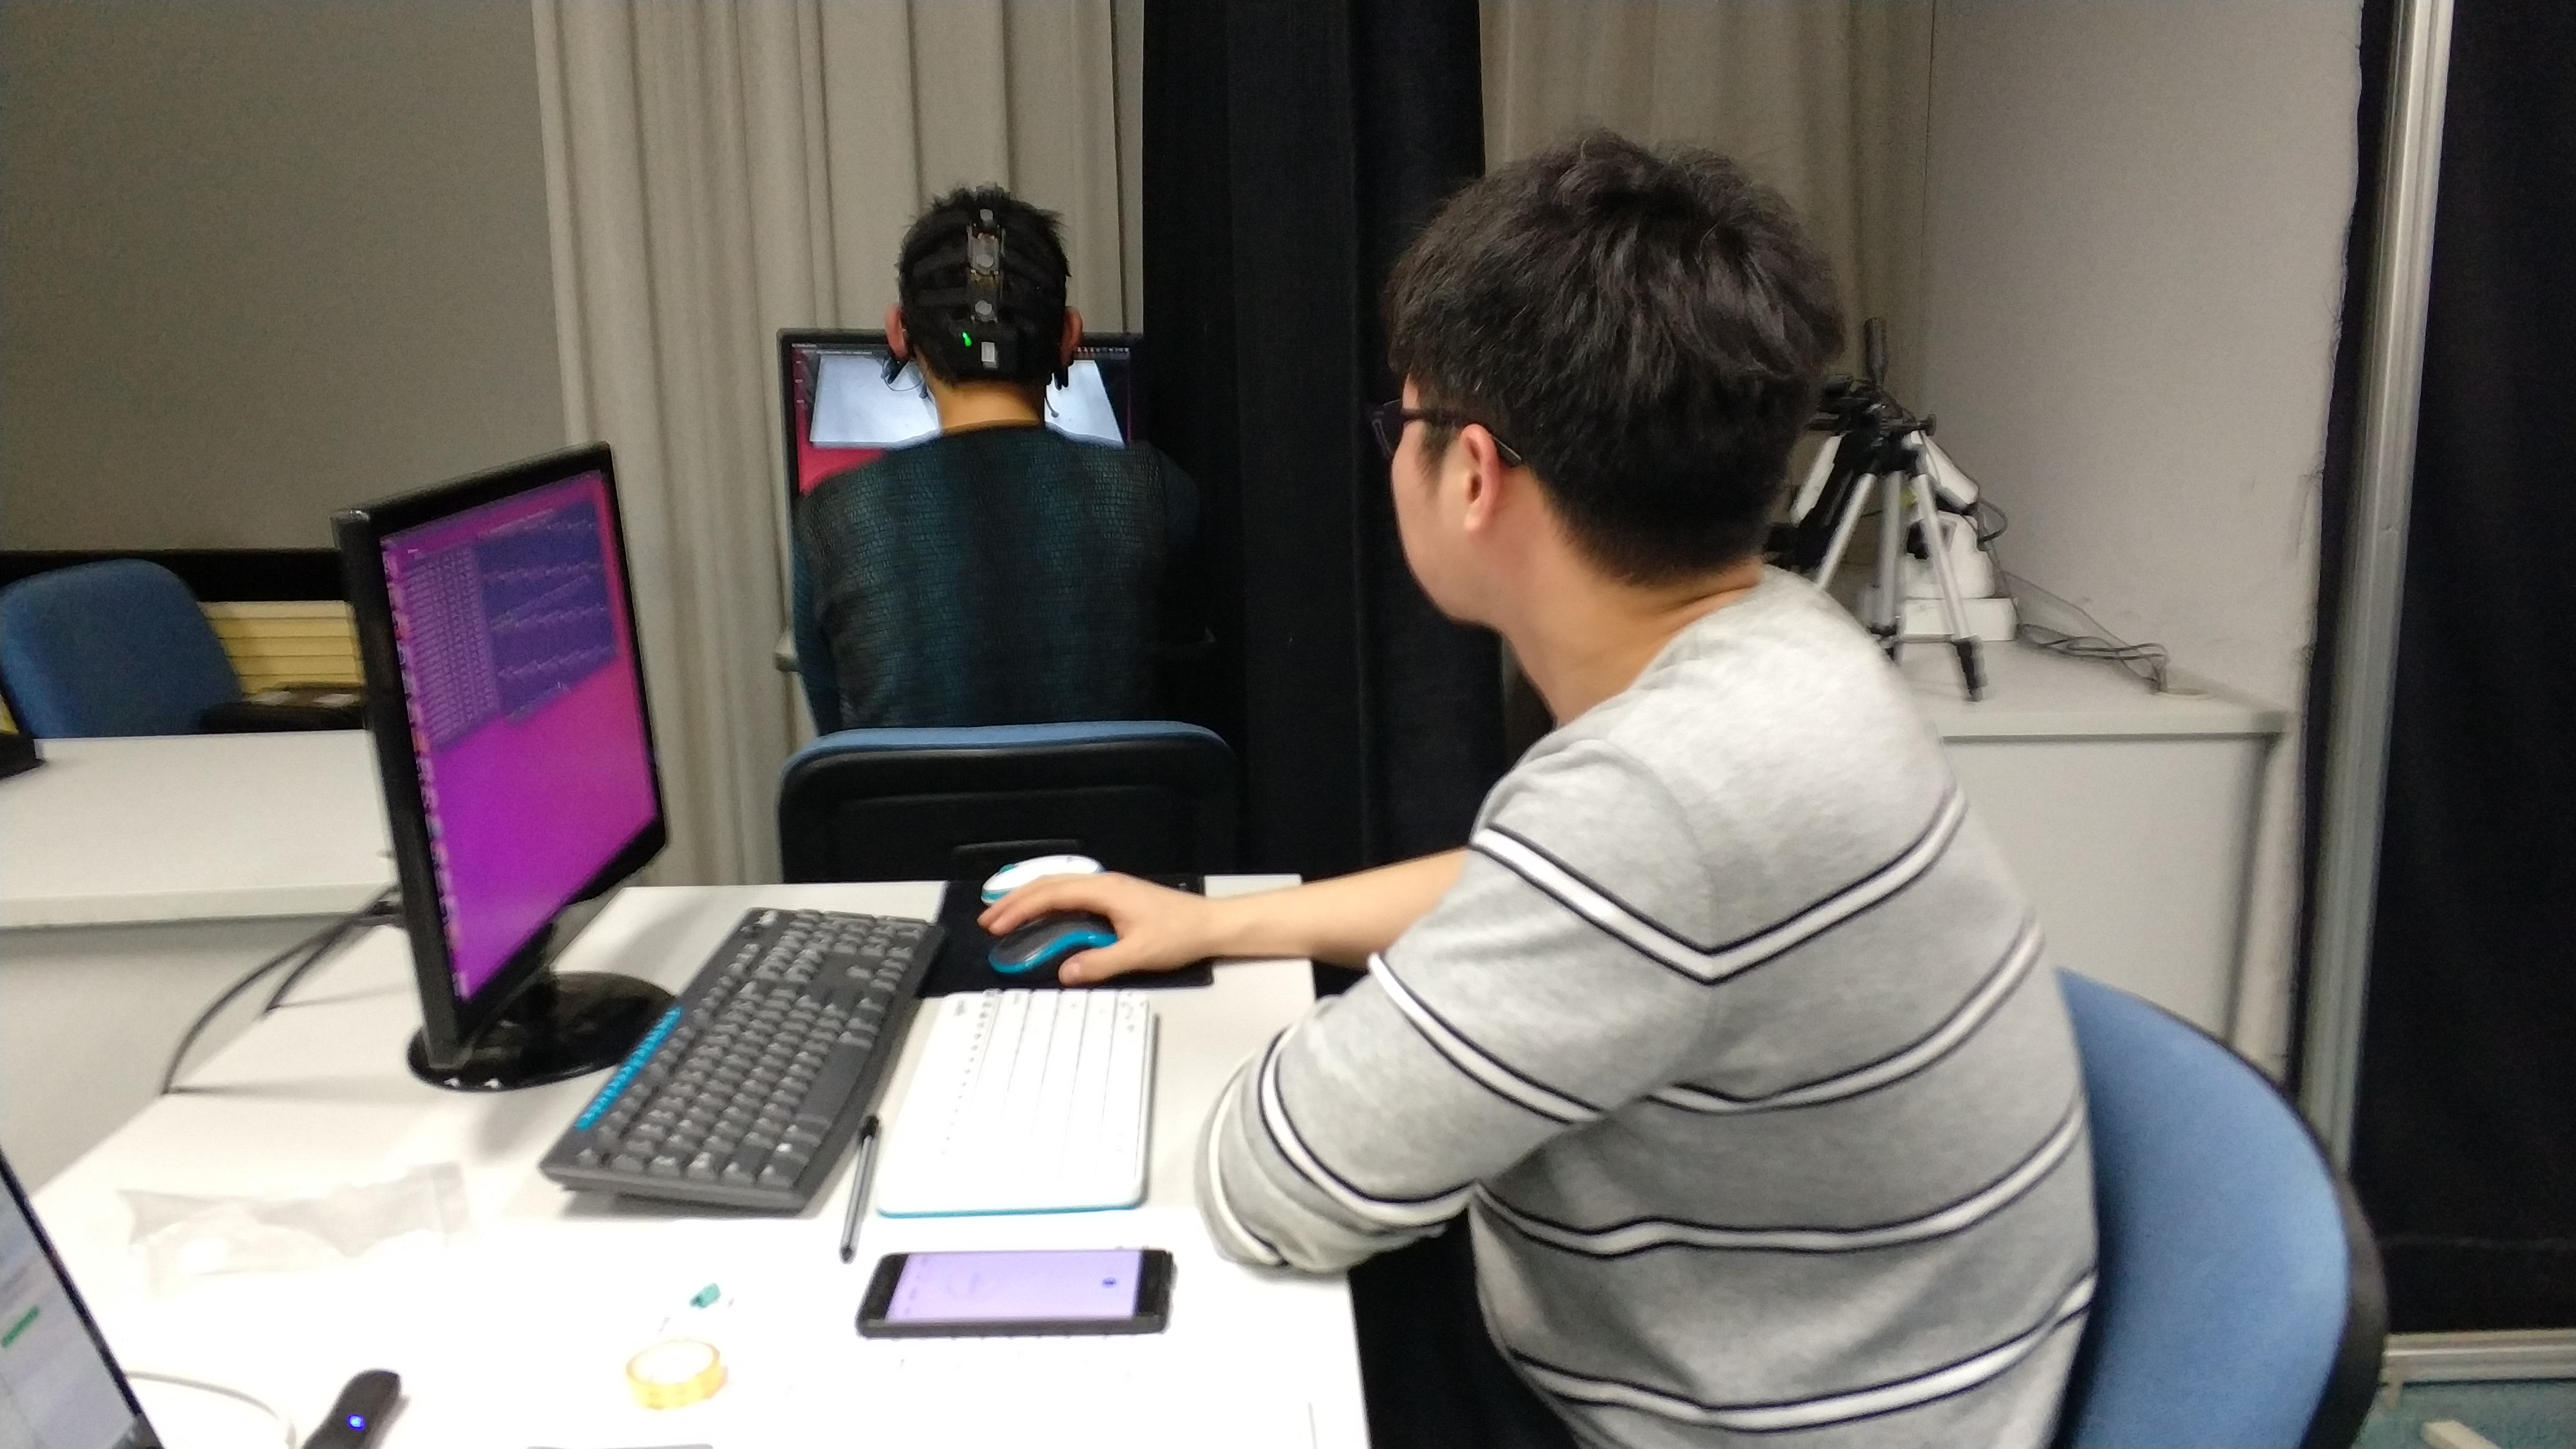
\includegraphics[width=1.5in]{images/5}}
  \hspace{0.5in}
  \subfigure[the subject operating joystick]{
    \label{fig:experiment:b} %% label for second subfigure
    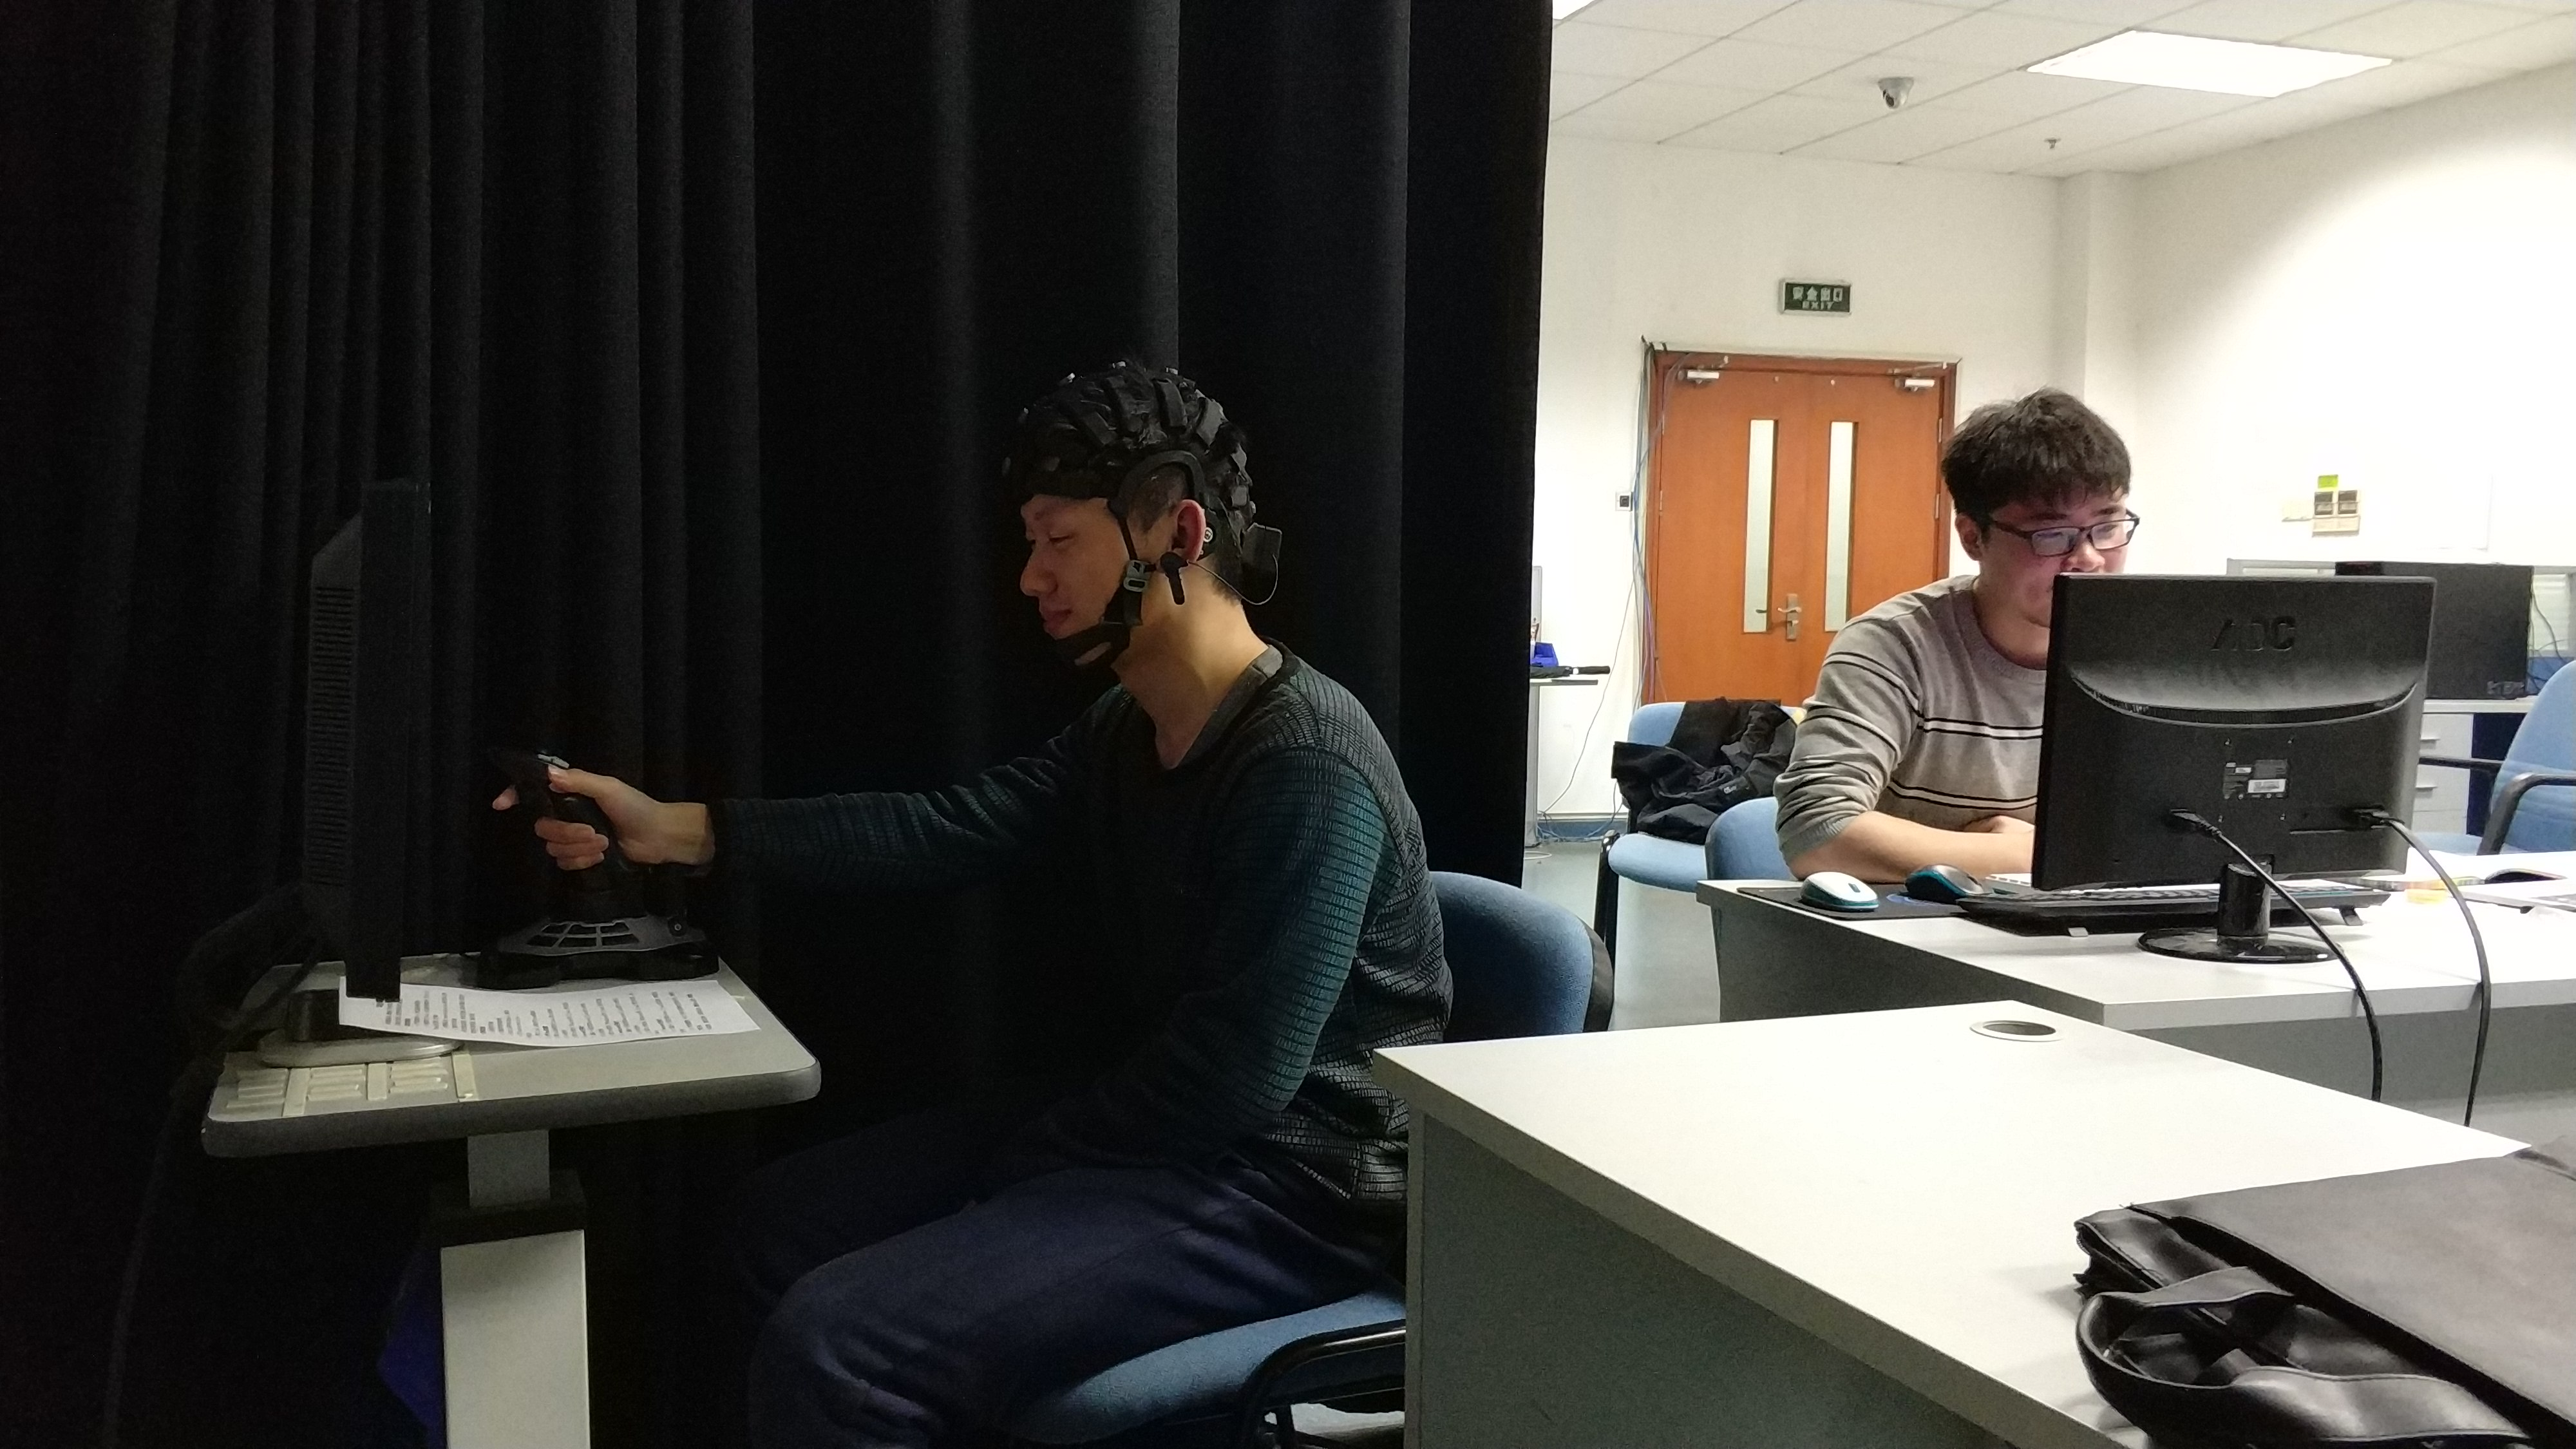
\includegraphics[width=1.5in]{images/6}}

  \subfigure[the mechnical arm operation platform]{
    \label{fig:experiment:c} %% label for second subfigure
    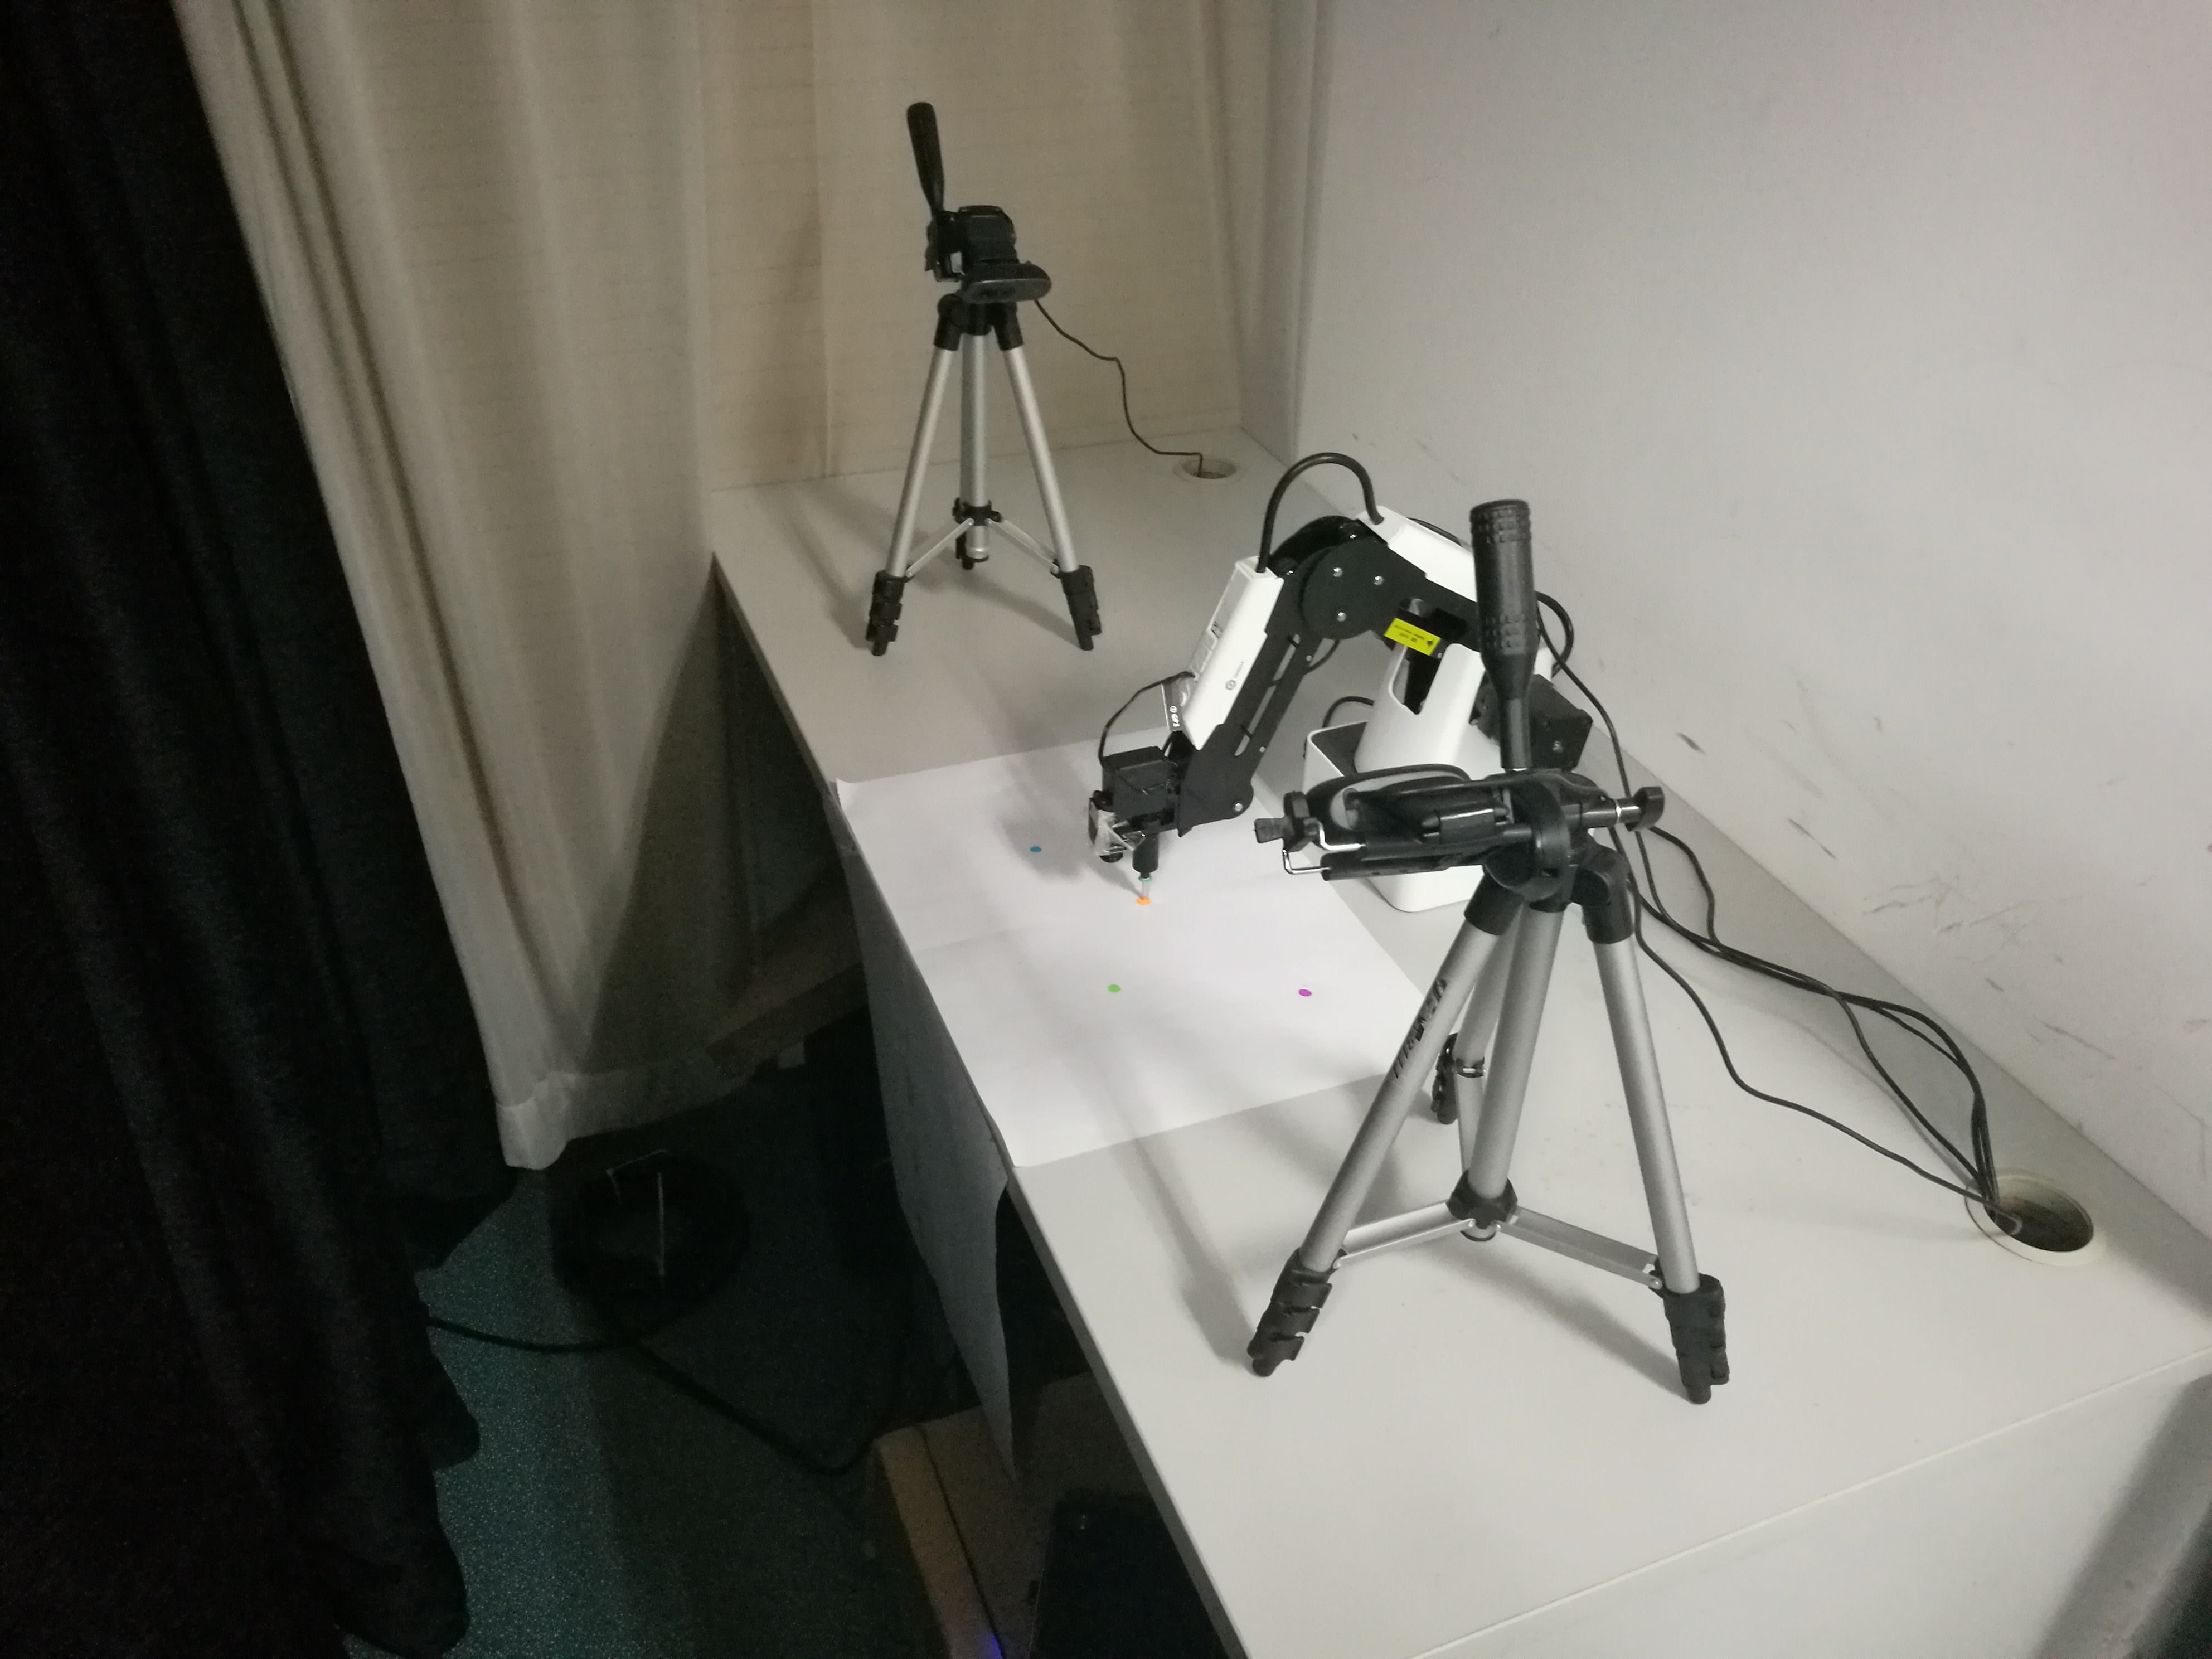
\includegraphics[width=1.5in]{images/7}}
  \hspace{0.5in}
  \subfigure[the screen showing camera information]{
    \label{fig:experiment:d} %% label for second subfigure
    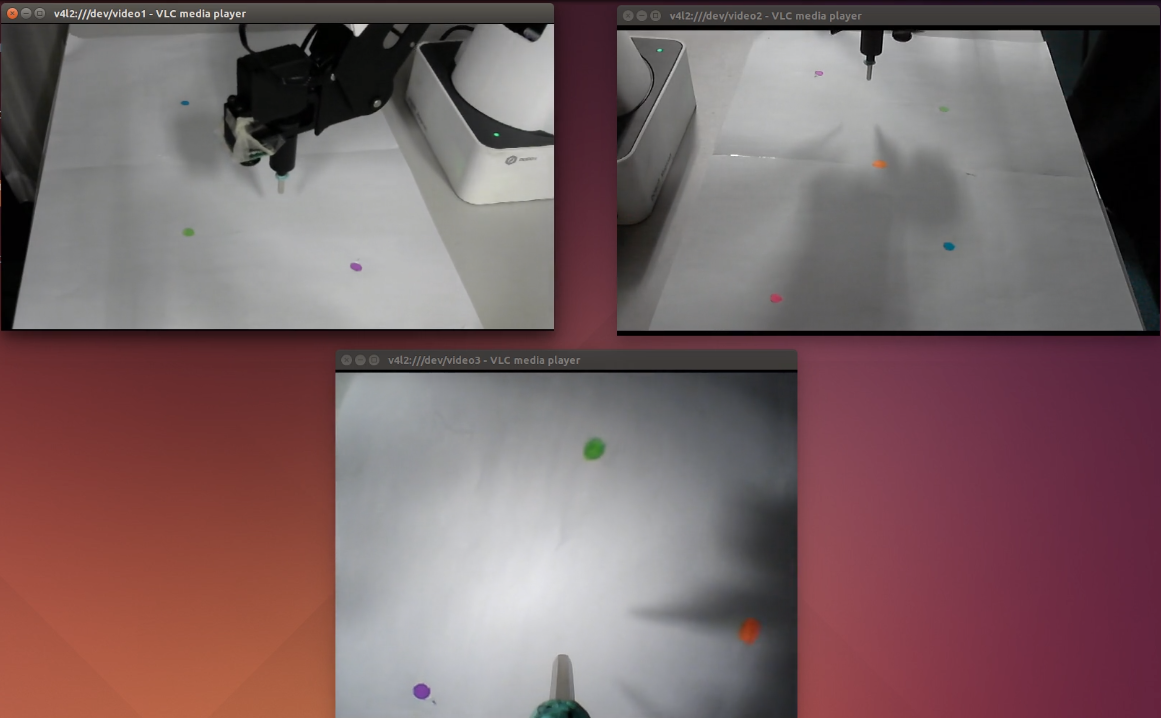
\includegraphics[width=1.5in]{images/8}}
  \caption{The experiment environment}
  \label{fig:experiment} %% label for entire figure
\end{figure}

\section{Data Preprocess Methods}
In data science field, data preprocess is the key procedure before any data analysis
procedure. The quality of data preprocess directly affects the final accuracy of
recognition. In EEG experiment, beacuse of the low signal noise rate (SNR) and
various interference, filtering and amplifying EEG signal is a crucial step before
EEG data analysis. And in our experiment, we need to do some label data preprocess
to obtain more objective real time label of EEG data because of the use of sliding window which would
be mentioned in Section 4 and the need of combining self-assessment with objective data.

\subsection{EEG Data Preprocess}
For one subject experiment, the raw data are drawed in Fig.~\ref{fig:wave:a}.
And then according to the track mark and EEG signal mark, the EEG signal and
the track were aligned in time. And we divided the entire EEG signal to
easy mode, medium mode and hard mode procedure according to the mark information.
The divided easy mode raw data, as an example, are showed in Fig.~\ref{fig:wave:b}.
Next, to remove the disturbance of EMG signal and the interference of various
electromagnetic signal which are generally high frequecy signals, we use band
filter to filter out 1-64Hz signal, which are the dominant frequency band of EEG
signal(see in Fig.~\ref{fig:wave:c}). Because the EEG signal has extra low SNR,
the filtered signal at the beginning and end part is unstable. Therefore we selected
to remove the first and last 5 seconds data (see in Fig.~\ref{fig:wave:d}).
And for the computing convenience, the selected data are normalized to [-1,1] area
according to all 32 channels signal by min-max normlization.

\begin{figure}
  \centering
  \subfigure[raw data]{
    \label{fig:wave:a} %% label for a subfigure
    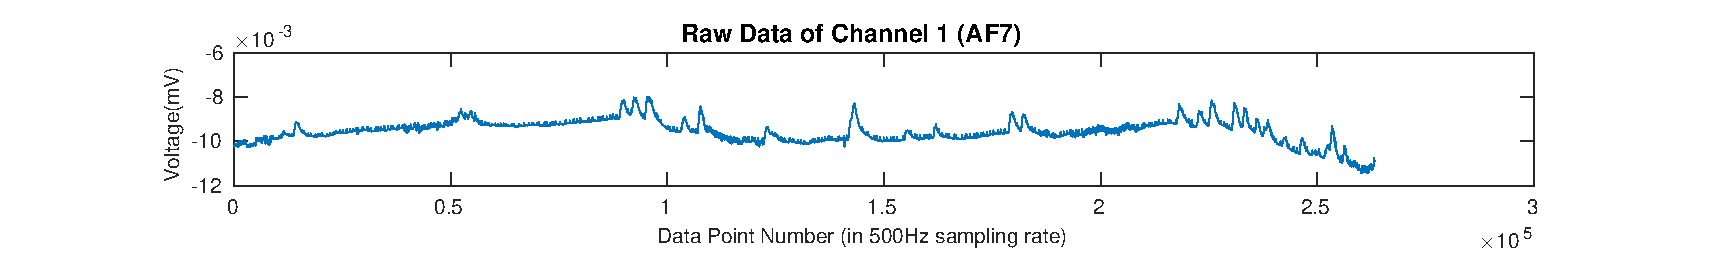
\includegraphics[width=4in]{images/9}}

  \subfigure[easy mode raw data]{
    \label{fig:wave:b} %% label for b subfigure
    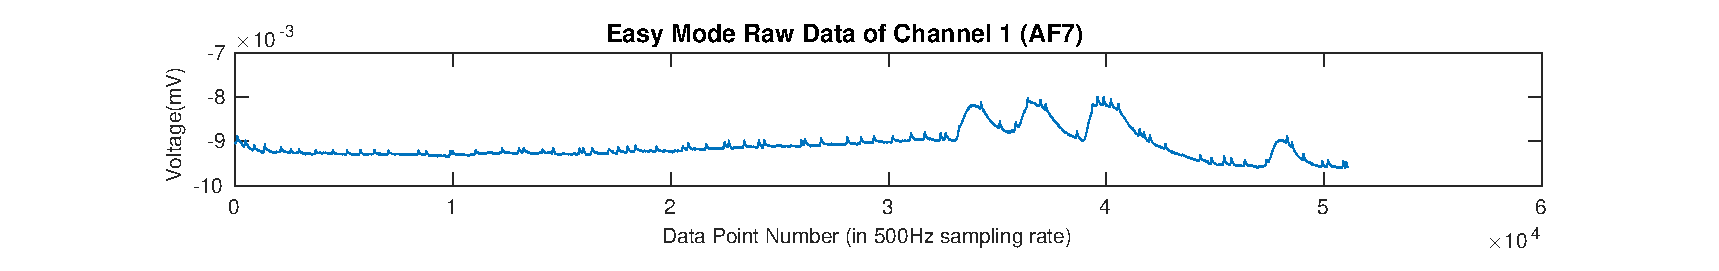
\includegraphics[width=4in]{images/10}}

  \subfigure[filtered data]{
    \label{fig:wave:c} %% label for c subfigure
    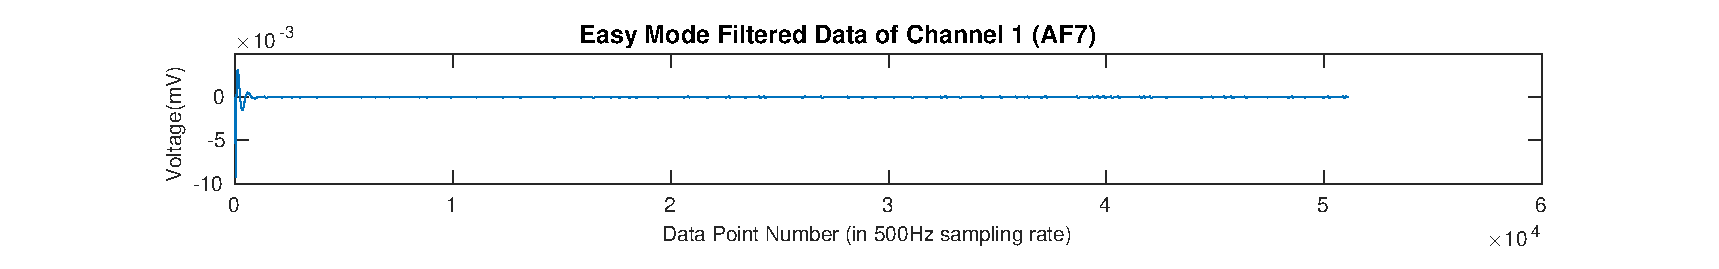
\includegraphics[width=4in]{images/11}}

  \subfigure[selected data]{
    \label{fig:wave:d} %% label for d subfigure
    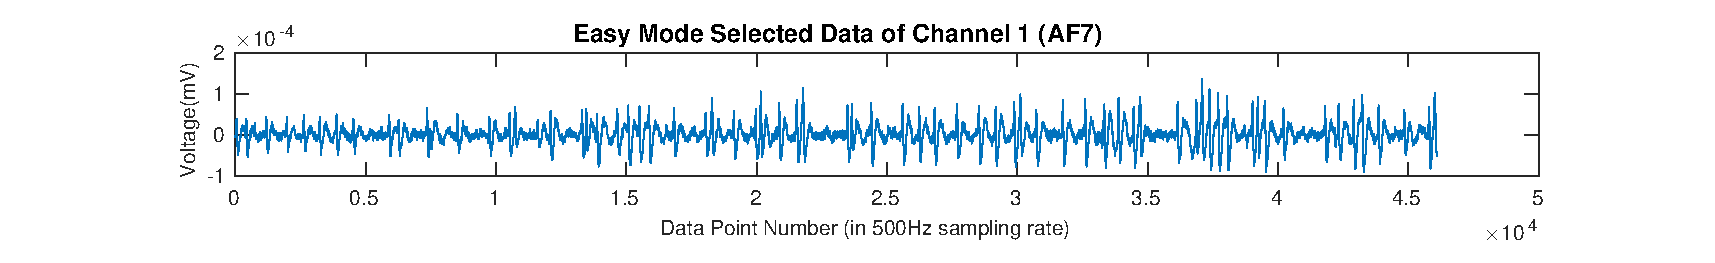
\includegraphics[width=4in]{images/12}}

  \subfigure[normalized data]{
    \label{fig:wave:e} %% label for e subfigure
    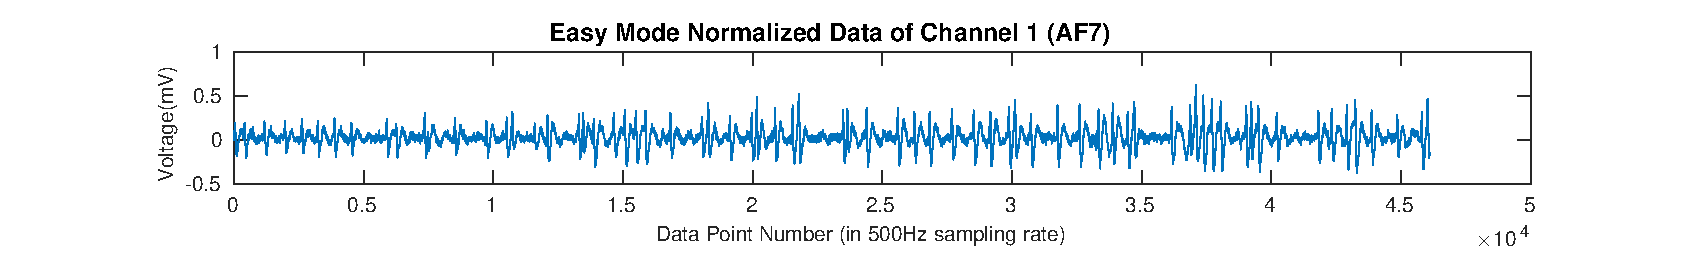
\includegraphics[width=4in]{images/13}}
  \caption{Data preprocess wave charts}
  \label{fig:wave} %% label for entire figure
\end{figure}

\subsection{Label Data Preprocess}
Label data includes three parts in total: the self-assesment of subjects, the difficulty
level experimenters design and the performance the track reflects. The self-assesment
is the subjective label data and the difficulty level and the performance are the
objective data.

For the self-assesment, after the entire experiment were finished,
each subjects were asked to fill a table about their emotion state during
operating different tasks. There were seven level the subjects could choose.
"1" means the most positive emotion state, "4" means neutral emotion state and
"7" means the most negative emotion state. The greater the number, the worse the
emotion state. And then we used each score to weighted each task.

For the the difficulty level experimenters desgin, we simply gave the scores of
difficulty according to the workload and the time pressure. In easy task, we
asked the subjects to touch three points without time constraint, which means that
we assumed the most positive emotion state could be stimulated by this task.
On the contrary, in hard task, we asked the subjects to touch five points with a ninety seconds
constraint, which means that we assumed the most negtive emotion state could be stimulated by
this task. We used "2.5", "4" and "5.5" to represent the emotion states different difficulty levels
we assumed could stimulate.

For the performace, we recorded the tip trajectory of mechnical arm. As showed
in Fig.~\ref{fig:track}, in easy mode, the subjects were asked to touch orange
point, purple point and pink point in order from a random start point. We assumed
that the subjects would feel positive when they moved the mechnical arm smoothly,
so we counted the numbers of direction change, in selected sliding window
mentioned in Section 4, as the estimation of the emotion state of the subjects.

\begin{figure}
  \centering
  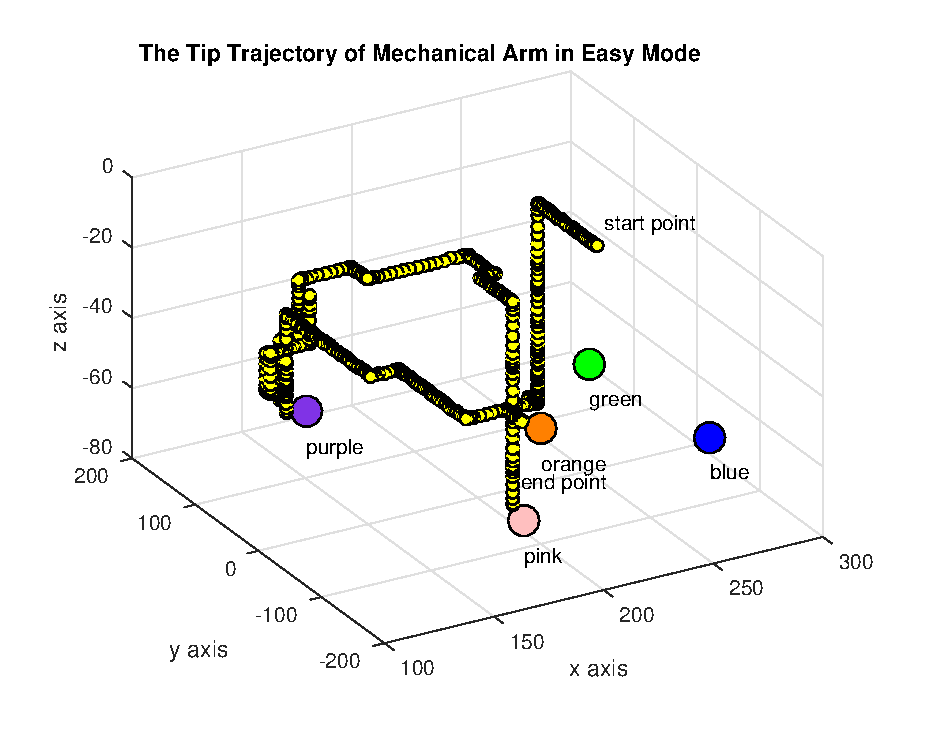
\includegraphics[height=6cm]{images/14}
  \caption{The tip trajectory of mechnical arm in easy mode}
  \label{fig:track}
\end{figure}

We use the formula below to caculate the final label.

\begin{equation}
  L = \frac{1}{3}(L_{self-assessment}) + \frac{1}{3}(L_{difficulty-level}) +
      \frac{1}{3}(L_{direction-change})
\end{equation}
where $L_{self-assessment}$ means the self-assessment score, $L_{difficulty-level}$
 means the difficulty level score, $L_{direction-change} = 3\frac{N_{direction-change} - N_{min}}
{N_{max} - N_{min}} - 1.5$ means the direction change score, among them,
$N_{direction-change}$ means the number of direction changes,
$N_{min}$ means the minium of $N_{direction-change}$ and
$N_{max}$ means the maxium of $N_{direction-change}$.

\section{Affective Recognition Methods}
Traditional pattern recognition process includes 4 steps: data preprocess,
feature extraction, feature selection and classification design. In this paper,
we use several classic methods in feature extraction, feature selection
and classification design procedure to explore their performance in
our experiment data.

\subsection{Multi-scale Feature Extration}
The multi-scale feature extraction procedure are divided in two steps:
1) sliding window selection and
2) feature extraction.

\paragraph{\textbf{\emph{Sliding Window Selection}}}

Because uncertain relation between time interval and emotion state change,
we chose 2s, 4s, 6s, 8s, 10s as the length of sliding window and 0.2s
as the length of stride to extract multi-scale features.

\paragraph{\textbf{\emph{Feature Extraction}}}
According to the paper\cite{Feature}, we chose 18 dimensions time domain features,
which are statistical features,
higher order crossings (HOC) features and fractal dimension feature, and 53
dimensions frequency domain features, which are band power, bin power and
the ratio of mean band powers $\beta/\alpha$.

\emph{Time Domain Features}

In this paper, we chose seven \emph{statistical\ features} to represent the
raw EEG time series. There are:

a) Mean: ${\mu}_{\bm{\eta}} = \frac{1}{T}\sum_{t=1}^T \bm{\eta}(t)$

b) Power: $P_{\bm{\eta}} = \frac{1}{T}\sum_{-\infty}^{\infty} |{\bm{\eta}}(t)|^2 $

c) Standard deviation: $\sigma_{\bm{\eta}} = \sqrt{ \frac{1}{T} \sum_{t=1}^{T-1} ({\bm{\eta}}(t) - {\mu}_{\bm{\eta}})^2 }$

d) 1st difference: $\delta_{\bm{\eta}} = \frac{1}{T-1}\sum_{t=1}^{T-1}|{\bm{\eta}}(t+1) - {\bm{\eta}}(t)|$

e) Normalized 1st difference: $ \bar{\delta_{\bm{\eta}}} = \frac{ \delta_{\bm{\eta}}}{\sigma_{\bm{\eta}}}$

f) 2nd difference: $\gamma_{\bm{\eta}} = \frac{1}{T-2}\sum_{t=1}^{T-2}|{\bm{\eta}}(t+2) - {\bm{\eta}}(t)|$

h) Normalized 2nd difference: $\bar{\gamma_{\bm{\eta}}} = \frac{\gamma_{\bm{\eta}}}{\sigma_{\bm{\eta}}}$

To find more robust features and pattern of EEG, Petrantonakis and Hadjileontiadis proposed
 higher order crosssings (HOC) features\cite{HOC}. Therefore we applied \emph{HOC} to represent the raw EEG time series.
The higher order series could be caculated by the formula below:
\begin{equation}
    H_k\{{\bm{\eta}}(t)\} = \nabla^{k-1}{\bm{\eta}}(t)
\end{equation}
where $\nabla$ means ${\bm{\eta}}(t) - {\bm{\eta}}(t-1)$. Therefore, the features
of HOC could be caculated by counting the sign changes or equation below:
\begin{equation}
  F_k = \sum_{t=1}^{T-k}\psi(H_k\{{\bm{\eta}}(t)\}H_k\{{\bm{\eta}}(t+1)\}), k = 1,2...10
\end{equation}
where $\psi(t)$ is a section function which is defined below:

\begin{equation}
   \psi(x)=
   \begin{cases}
   0 &\mbox{if x $\geq$ 0}\\
   1 &\mbox{if  x $<$ 0}
   \end{cases}
\end{equation}

The fractal dimention (FD) as a feature measuring the complexity is widely used.
There are many mehtods computing the FD feature. In this paper, we chose to use
the Higuchi algorithm\cite{FD} to caculate the FD feature. To compute the FD
feature, the EEG series is rewritten as:
\begin{equation}
    \{{\bm{\eta}}(p), {\bm{\eta}}(p+q), {\bm{\eta}}(p+2q), ... , {\bm{\eta}}(q+[\frac{T-q}{q}]q)\},\ p = 1,2,...,q
\end{equation}
where [x] means the largest integer less than x. Then we could define the series $M_p(q)$ as below:
\begin{equation}
  M_p(q) = \frac{T-1}{[\frac{T-p}{q}]q^2}\sum_{k=1}^{[\frac{T-p}{q}]}|{\bm{\eta}}(p+kq) - {\bm{\eta}}(p+(k-1)q)|
\end{equation}
 Therefore we could further define the average:
\begin{equation}
  F(q) = \frac{1}{N_p}\sum_{p=1}^{N_p}M_p(q)
\end{equation}
where $N_p$ means the maxium of p.
According to paper\cite{FD}, we knew that $F(p)$ is proportional to $p^{-F_{FD}}$
(where $F_{FD}$ means the feature of FD). Therefore we could assumed:
\begin{equation}
   F(q) = r\cdot{p^{-F_{FD}}}
\end{equation}
when we log the equation, we could obtain:
\begin{equation}
  log(F(q)) = log(r) - {F_{FD}}log(p)
\end{equation}
Therefore we could obtain FD feature $F_{FD}$ by the slope of $log(F(q))$ to $log(p)$.

\emph{Frequency Domain Features}

For time series signal, spectrum analysis is an important method extracting features.
Through short-time fourier transform (STFT)\cite{STFT}, which is a more robust method,
we could get the power value as a function of time and frequecy: $P(t,f)$.
A
\subsection{Feature Selection}
\subsection{Classification}

\section{Results}

\section{Discussion}

\section{Conclusion}



\begin{thebibliography}{4}

\bibitem{AC} Picard R W.
  Affective computing[M].
   MIT Press, 1997.

\bibitem{KR} Khosrowabadi R, Wahab A, Ang K K, et al.
Affective computation on EEG correlates of emotion from musical and vocal stimuli[C]
//Neural Networks, 2009. IJCNN 2009. International Joint Conference on. IEEE, 2009: 1590-1594.

\bibitem{Ekman} Ekman P, Friesen W V, O'sullivan M, et al.
Universals and cultural differences in the judgments of facial expressions of emotion[J].
Journal of personality and social psychology, 1987, 53(4): 712.

\bibitem{Plutchik} Plutchik R.
Emotions: A general psychoevolutionary theory[J].
Approaches to emotion, 1984, 1984: 197-219.

\bibitem{Russell} Russell J A.
A circumplex model of affect[J].
Journal of personality and social psychology, 1980, 39(6): 1161.

\bibitem{Feature} Jenke R, Peer A, Buss M.
Feature extraction and selection for emotion recognition from EEG[J].
IEEE Transactions on Affective Computing, 2014, 5(3): 327-339.

\bibitem{cognionics} Documents of The Cognionics HD-72 Dry EEG,
\url{http://www.cognionics.com/images/docs/HD72.pdf}

\bibitem{dobot} Specification of The Dobot Magician mechnical arm,
\url{https://www.dobot.cc/dobot-magician/specification.html}

\bibitem{joystick} Features of The Extreme 3D Pro joystick,
\url{https://www.logitechg.com/en-us/product/extreme-3d-pro-joystick#featuresAnchor}

\bibitem{HOC} Petrantonakis P C, Hadjileontiadis L J.
Emotion recognition from EEG using higher order crossings[J].
IEEE Transactions on Information Technology in Biomedicine, 2010, 14(2): 186-197.

\bibitem{FD} Liu Y, Sourina O.
Real-time fractal-based valence level recognition from EEG[M]
//Transactions on Computational Science XVIII. Springer, Berlin, Heidelberg, 2013: 101-120.

\bibitem{STFT} Lin Y P, Wang C H, Jung T P, et al.
 EEG-based emotion recognition in music listening[J].
 IEEE Transactions on Biomedical Engineering, 2010, 57(7): 1798-1806.
\end{thebibliography}

















\end{document}
